
\chapter{Implementierung}
\label{chap:impl}
\todo[size=\small, color=yellow!40, inline]{Needs Machine proofreading}%
\todo[size=\small, color=yellow!40, inline]{Needs Tim understanding}%
\todo[size=\small, color=yellow!40, inline]{Needs Non-Tim understanding}%
\todo[size=\small, color=yellow!40, inline]{Needs Human proofreading}%

In dieser Arbeit wurde ein paralleles Out-Of-Core-Rendering System entwickelt, welches auf einem hybriden Linux-Cluster arbeitet. Dazu wurde kein bestehendes System erweitert, sondern ein eigenes System von Grund auf neu entwickelt. Als Programmiersprache wurde C++ mit verschiedenen Programmbibliotheken verwendet; unter anderem OpenGL, boost und OpenMPI \cite{mpi}. An wird erläutert, wie das System funktioniert.\\

\section{Preprocessing}
\label{sec:impl:preprocessing}
Das Modell der Boeing 777 liegt im OBJ-Format\footnote{Ein freies nicht-binäres Dateiformat zur Beschreibung von Geometrie. \cite{obj}. } vor. Eine Textdatei zu parsen und zu laden ist wesentlich langsamer als dieselben Daten binär auszulesen, da die Daten erst von Text in Zahlen konvertiert werden müssen. Räumliche Datenstrukturen sind ebenfalls nicht vorhanden. Aus diesem Grund ist es notwendig, diese 3D-Szene zuvor in ein Format zu übertragen, welches einfacher und schneller zu handhaben ist. Viele Rendering-Systeme bauen räumliche Datenstrukturen wie Octrees beim Programmstart ad hoc auf. Das ist im Falle der Boeing nicht praktikabel, da das Modell nicht in den Speicher passt.

Das Preprocessing fasst eine Menge an Vorberechnungen zusammen, die danach nie wieder durchgeführt werden müssen. Zunächst mussten die OBJ-Dateien bereinigt werden, da an vielen Stellen Sonderzeichen verwendet wurden, die vielen kommerziellen 3D-Modellierungsprogrammen Probleme bereiten. Als geometrische Primitive gab Polygone mit über 24 Eckpunkten. Um die VBOs rendern zu können, ist es jedoch erforderlich, dass ausschließlich Dreiecke verwendet werden. Diese Polygone mussten zuerst in Dreiecke umgewandelt werden. \\
Die Farben waren in Form einer Exceltabelle gegeben, welche zunächst in OBJ-Konforme Materialbeschreibungen umgewandelt wurden. Anschließend wurden die Objekte in ein binäres Format konvertiert, in dem die Vertices und Normalvektoren eines Objektes direkt hintereinander in einer Datei standen. Die Farben wurden zu einer 1D-Farbtextur zusammengefasst und die entsprechende Texturkoordinate als vierte Komponente in den Vertices gespeichert (siehe \ref{sec:basics:computergrafik}). Für den Aufbau des Loose Octrees wurde versucht, die Octree-Struktur in Form von Unterverzeichnissen auf dem Datenträger abzubilden. Die Objekte wurden einzeln in die Wurzel eingefügt und bei Überschreiten des Dreieckslimits von 5.000 Stück pro Knoten weiter aufgeteilt. Dadurch wurde jedoch die Grenze an Unterverzeichnissen in einem Verzeichnis von ca. 32000 überschritten. Eine Verzeichnisauflistung dauerte mehr als 30 Minten. Aus diesem Grund wurden alle Datenobjekte im Octree mit Indizes versehen und das Skelett des Octrees in einer separaten Datei gespeichert. Anschließend wurden alle Objekte in 500 MiB Dateiblöcken zusammengefasst. Mit dem Octree-Skelett lässt sich die Struktur des Baums laden, ohne tatsächlich Objektdaten darin speicher zu müssen. Dafür sind alle Informationen über Anzahl der Dreiecke, ID des Knotens, Baumtiefe und Vielem mehr, direkt abrufbar.

Der Rechenaufwand für das Preprocessing hat auf einen Dual Core AMD Opteron mit 2.4 GHz und 3 GiB RAM zusammengerechnet ca. 50 Stunden reine Rechenzeit benötigt. An der Zeit lässt sich erkennen, dass es von Vorteil ist, die Datenstruktur auf Festplatte zu speichern, da sich der fertig aufgebaute Octree wesentlich schneller laden lässt, als ihn aufzubauen.

\section{Netzwerkarchitektur}
\label{sec:impl:netzwerkarchitektur}
Als Testumgebung wurde der der Arminius-Custer im Paderborn Center for Parallel Computing \cite{pc2} genutzt. Das System besteht aus zwei verschiedenen Rechnertypen: den Visualisierungsknoten und den Rechenknoten. In Tabelle \ref{tab:impl:arminius} lassen sich die einzelnen Komponenten der beiden Knotentypen vergleichen. Da die Rechenknoten schwächere Grafikkarten besitzen, wird das eigentlich Rendering auf den Visualisierungsknoten durchgeführt. Die Datenknoten rendern lediglich die sichtbaren Objekte ohne Beleuchtung und Schattierung in ihre Tiefenbuffer.\\
Ursprünglich befand sich die 3D-Szene auf einem verteilten Dateisystem, was sich jedoch als Problem herausstellte, da die Dateigrößen und deren Inhalt nicht immer korrekt gelesen werden konnten. Wenn allerdings 32 Datenknoten gleichzeitig auf dieselben Daten zugreifen, dauert der Ladevorgang über 5 Stunden. Deshalb liest ein Knoten jede Datei ein und verschickt diese über das InfiniBand Netzwerk, was den Ladevorgang auf ca. 10 Minuten beschleunigt. Die Tests wurden dabei auf 2 Visualisierungsknoten und 24, 28 und 32 Rechenknoten durchgeführt.

\begin{table}
 \centering
 \begin{tabular}{lll} % die ersten beiden Spalten linkbündig, die letzte zentriert
  \toprule % die linienbegrenzungen
  \textit{Komponente} & \textit{Rechenknoten} & \textit{Visualiserungsknoten} \\
  \midrule
  \textbf{Betriebssystem} & Linux & Linux \\
  \textbf{Prozessor} & Dual INTEL Xeon 3.2 GHZ & Dual AMD Opteron 2.2 GHz \\
  \textbf{RAM} & 4 GByte & 8 GByte \\
  \textbf{Grafikkarte} & nVidia Quadro NVS 280 & nVidia Quadro FX 4500 PCI-e \\
  \textbf{Netzwerk} & InfiniBand 4x (10GBit/sec) & InfiniBand 4x (10GBit/sec) \\
  \bottomrule
 \end{tabular} 
 \caption{Konfiguration des Arminius-Clusters}
 \label{tab:impl:arminius}
\end{table}

\section{Rendering-Algorithmus}
\label{sec:impl:renderalgo}

Das System ist in drei verschiedene Prozesstypen unterteilt. Ein Masterknoten dient in erster Linie als Schnittstelle zwischen dem Benutzer und dem System. Mehrere Renderknoten kümmern sich um die Erzeugung einer Bildkachel. Viele Datenknoten überprüfen angeforderte Objekte auf deren Sichtbarkeit und verschicken die Daten gegebenenfalls über das Netzwerk. Alle Prozesse laufen so lange in einer Schleife, bis das Programm beendet wird. Jeder Schleifendurchlauf bei einem Render- oder Masterknoten entspricht einem Frame.\\
Der Master reagiert auf Eingaben und zeigt das vollständig gerenderte Bild an. Der Master hat aber auch die Aufgabe, die 3D-Szene zu Beginn eines Programmlaufs an alle Rechenknoten zu verschicken und das $c$-Collision Protokoll durchzuführen (siehe \ref{sec:basics:daten}). In Pseudocode \ref{alg:impl:masternode} ist das Prinzip des Masterknotens als Pseudocode dargestellt. Eingaben über Maus und Tastatur werden über ein Eventsystem bearbeitet, sobald sie anfallen. Ereignisse, die an andere Prozesse verschickt werden müssen, wie beispielsweise das Umschalten auf eine Wireframe-Darstellung, werden gesammelt und zu Beginn der Programmschleife verschickt. Jeden Frame wird ein Frame-Counter erhöht und nach 20 Frames, in denen die Kamera bewegt wurde, ordnet der Master eine Erneuerung des Tiefenbuffers der Datenknoten an. Im Zuge dessen werden auch die Kachelgrößen der Renderknoten angepasst, da sich dabei die Framebuffer-Dimension bei den Datenknoten auch ändert und ohnehin ein neuer Tiefenbuffer benötigt würde. Anschließend wartet der Master auf eintreffende Objektanfragen von den Renderknoten, um anhand des $c$-Collsion Protokolls die Auftragsvergabe an die Datenknoten zu ermitteln.
\begin{figure*}[ttt!]
\centering
 \begin{minipage}[t]{12cm}
\begin{algorithm}[H]
  \floatname{algorithm}{Pseudocode}
  \caption{MasterNode (auf Visualisierungsknoten)\label{alg:impl:masternode}} 
    \begin{algorithmic} [1]
      \STATE \textbf{send} alle Objektdaten an alle Datenknoten
      \LOOP
	\STATE \textbf{send} Kameraposition und Eingaben an alle Renderer
	\IF{ Frame-Nummer $>$ Schwellwert}
	  \STATE Berechne neue Kachelgrößen
	  \STATE \textbf{send} Kachelgrößen an alle Renderknoten
	\ENDIF
	\STATE \textbf{wait} auf Datenanfragen von allen Renderknoten
	\STATE führe $c$-Collsion Protokoll auf Datenanfragen aus
	\STATE \textbf{send} Anfragen an ermittelte Datenknoten weiter
	\STATE \textbf{wait} auf Bildkacheln von allen Renderknoten
	\STATE rendere Bild und zeige es an
      \ENDLOOP
    \end{algorithmic}
\end{algorithm}
 \end{minipage}
%\caption{Der Pseudo-Code des Masterknotens.}
\end{figure*}

Um keinen Auftrag zu bevorzugen, wird die gesamte Menge an Aufträgen randomisiert. Das $c$-Collsion Protokoll wird dann auf einer Untermenge an Aufträgen durchgeführt, welche höchstens der Anzahl an Datenknoten entspricht. Mit jedem Auftrag ist eine Menge an Dreiecken verbunden, die in dem Objekt enthalten sind. Die Dreiecke dienen hierbei als Gewichtung. Sollte ein Auftrag im Verlauf des $c$-Collsion Protokolls an mehrere Datenknoten vergeben werden können, wird zufällig ermittelt, welche der infrage kommenden Knoten den Auftrag erhält. Die bisher vergebene Zahl an Dreiecken an einen Knoten dient dabei als Gewichtung zur Beeinflussung dieser Verteilung, damit alle Knoten möglichst gleich ausgelastet sind.\\
Sei $n$ die Anzahl an Datenknoten, die für ein bestimmtes Objekt zuständig sind und $t_i$ die Anzahl der Dreiecke eines Knotens $i$. Dann ist
\[T=\sum_{i=0}^{n} \left(t_i\right)\]
die Summe der bisher vergebenen Dreiecke all dieser Knoten. Die Wahrscheinlichkeit $p_k$, dass ein Knoten $k$ zur Bearbeitung des Auftrags ausgewählt wird, beträgt somit 
  \[p_k=\frac{T-t_k}{\sum_{j=0}^{n} \left(T-t_j\right)}.\]
Gibt es zum Beispiel 3 Knoten $N_0,\; N_1,\; N_2$ die ein bestimmtes Objekt besitzen, mit einer Last von je 10, 1 und 89 bisher erhaltenen Dreiecken, so ergeben sich die Wahrscheinlichkeiten
\[p_0=\frac{100-10}{200}, \;p_1=\frac{100-1}{200}\; und \;p_2=\frac{100-89}{200}\]
für diese Knoten. Sollten nicht alle Aufträge mit dem anfänglichen $c=2$ vergeben werden können, wird das $c$ erhöht. Nachdem alle Aufträge eines Frames vergeben wurden, wird die akkumulierte Last wieder zurückgesetzt. Die ermittelte Auftragsverteilung wird danach an die Datenknoten geschickt.\\
Anschließend wartet der Master auf die Bildkacheln von allen Renderern und zeigt das fertige Bild an.

Ein Renderknoten (siehe Pseudocode \ref{alg:impl:rendernode}) misst die Zeit, die ein Programmschleifendurchlauf dauert. Zu Beginn der Schleife werden Eingaben vom Master empfangen. Falls eine Tiefenbuffer-Aktualisierung angeordnet wurde, überträgt jeder Renderknoten seine gemittelten Renderzeiten, damit der Master anhand dieser neue Kachelgrößen vergeben kann. Anschließend wird dann ein Rendering-Pass mit der neuen Framebuffergröße durchgeführt, damit der so entstandene Tiefenbuffer an alle Datenknoten übermittelt werden kann. Mit einem Frame Versatz wird die Bildkachel aus dem letzten Frame geschickt. Dieser Versatz fällt jedoch nicht auf. Nun traversiert jeder Renderer das Octree-Skelett. Dabei werden alle Octree-Zellen, die sich innerhalb des Frustums befinden, in einer Liste gespeichert. Alle Objekte der Liste werden nun angefordert, sofern sie nicht schon auf dem Renderer vorhanden sind. Diejenigen Objekte, die zwar vorhanden sind, jedoch nicht innerhalb des Frustums liegen, verbleiben im Arbeitsspeicher des Renderers, werden jedoch aus dem Grafik-RAM entfernt. Diese Offline-Objekte erhalten einen Zähler, der bei jeder Octree-Traversion erhöht wird. Ist ein Objekt mehr als 200 Frames Offline, wird es vollständig vom Renderer entfernt.\\
Der Renderknoten überprüft dann, ob Daten von den Datenknoten an ihn geschickt wurden. Ist dies der Fall, wird eine asynchrone Übertragung begonnen. Zum Schluss der Programmschleife müssen noch Objekte überprüft werden, die mehr als 20 Frames ihren Status nicht geändert haben, also von Online zu Offline oder anders herum. Diese werden mittels eines lokalen Occlusion-Tests auf Sichtbarkeit geprüft und ihr Status wird gegebenenfalls geändert.
 
\begin{figure*}[ttt!]
\centering
 \begin{minipage}[t]{12cm}
\begin{algorithm}[H]
  \floatname{algorithm}{Pseudocode}
  \caption{RenderNode (auf Visualisierungsknoten)\label{alg:impl:rendernode}} 
    \begin{algorithmic} [1]
      \LOOP
	\STATE \textbf{wait} auf Kamera und Eingaben vom Masterknoten
	\IF{neue Kachlgröße empfangen}
	  \STATE ändere Kachelgröße und Framebuffer
	  \STATE \textbf{send} aktuellen Tiefenbuffer an alle Datenknoten
	\ENDIF
	\STATE \textbf{send} Bildkachel vom letzten Frame an Masterknoten
	\STATE Octree/Sampletree-Traversion \& Frustum-Culling
	\STATE verwalte Daten-Cache
	\STATE \textbf{send} Datenanfragen an Masterknoten
	\STATE \textbf{recv} ggf. Objekte von Datenknoten
	\STATE rendere Szene
	\STATE Occlusion-Test auf Objekten mit abgelaufenem Zähler
      \ENDLOOP
    \end{algorithmic}
\end{algorithm}
 \end{minipage}
%\caption{Der Pseudo-Code eines Renderknotens.}
\end{figure*}
\todo[size=\small, inline]{Maximale Objektgröße, bzw. Verteilung ebd. ermitteln. $\rightarrow$ Diagramm? =)}
Durch das ständige Allozieren und Freigeben von Arbeitsspeicher für die Verwaltung der Objekte der Speicher fragmentierte, musste eine eigene Speicherverwaltung implementiert werden (siehe Kapitel \ref{sec:basics:speicher}). Diese reserviert sich zu Beginn des Programms 1 GiB RAM und bietet Methoden diesen Speicherbereich aufgeräumt zu halten. Da das \verb|malloc()| und \verb|free()| des Betriebssystems erheblich aufwendiger arbeitet, als eine eigene Speicherverwaltung, ist das Reservieren und Freigeben innerhalb des eigenen Speicherbereichs auch schneller.\\
Die Liste mit vorhandenen und fehlenden Daten jeden Frame mehrfach zu durchlaufen hat sich als problematisch herausgestellt. Diese Liste enthielt, in Abhängigkeit von der Kameraposition und der Frustumtiefe mehr als 40.000 Elemente. Dadurch wurden die betroffenen Renderknoten verlangsamt. Deshalb wurde die maximale Größe der Liste auf 15.000 beschränkt, wodurch solche Verzögerungen vermieden werden konnten.

Datenknoten (siehe Pseudocode \ref{alg:impl:datanode}) haben keine framegebundene Programmschleife, da sie nur bei Bedarf auf ankommende Anfragen reagieren. Beim Programmstart errechnen sich alle Datenknoten eine Teilmenge von Objekten aus dem Octree, für die sie im weiteren Programmverlauf zuständig sind. Wenn der Masterknoten alle Daten über das Netzwerk verschickt, speichern sich die Datenknoten ihre zugewiesenen Objekte und verwerfen den Rest. Jeder Datenknoten besitzt einen eigenen Framebuffer für jeden Renderer, da sich die Kacheln im Zuge des Prefetchings (siehe \ref{sec:basics:speicher}) überschneiden. In der Programmschleife der Datenknoten überwachen diese ihren Nachrichteneingang und reagieren nur, wenn eine Nachricht vorliegt. Besteht die Nachricht aus einer Menge an Anfragen, werden diese zunächst nach den Renderern sortiert, die die Anfragen gestellt haben. Anschließend werden für alle Renderer und für alle angefragten Objekte Occlusion-Tests durchgeführt. Da erst alle Occlusion-Tests durchgeführt werden, bevor das Ergebnis überprüft wird, ist davon auszugehen, dass bis dahin alle Ergebnisse vorliegen. Gegebenenfalls muss der Datenknoten darauf warten. Alle sichtbaren Objekte dieser Anfragen werden in die jeweiligen Tiefenbuffer gerendert und die Objekte daraufhin verschickt.
\begin{figure*}[ttt!]
\centering
 \begin{minipage}[t]{12cm}
\begin{algorithm}[H]
  \floatname{algorithm}{Pseudocode}
  \caption{DataNode (auf Rechenknoten)\label{alg:impl:datanode}} 
    \begin{algorithmic} [1]
      \STATE Berechne Objektzuweisungen
      \STATE \textbf{recv} Objektdaten vom Masterknoten
      \IF{Objekt in Objektzuweisung enthalten}
	\STATE Speichere Objekt im RAM
      \ELSE
	\STATE Verwerfe Objekt
      \ENDIF
      \WHILE{running}
	\STATE \textbf{wait} ggf. auf eingehende Nachrichten
	\IF{Nachricht $=$ Datenanfrage}
	  \STATE sortiere Anfragen nach Renderknoten
	  \FORALL{Renderknoten}
	    \STATE führe Occlusion-Tests der Objektanfragen auf Boundingboxen aus
	  \ENDFOR
	  \FORALL{sichtbare Daten aus Anfragen}
	    \STATE rendere Objekt in Tiefenbuffer
 	  \ENDFOR
	  \STATE \textbf{send} sichtbare Daten gebündelt an entsprechende Renderknoten
	\ELSIF{Nachricht $=$ Tiefenbuffer}
	  \STATE schreibe Tiefenbuffer in Framebuffer des jeweiligen Renderknotens
	\ELSE \STATE\textbf{sleep}
	\ENDIF
      \ENDWHILE
    \end{algorithmic}
\end{algorithm}
 \end{minipage}
%\caption{Der Pseudo-Code eines Datenknotens.}
\end{figure*}

\section{Kommunikation}
\label{sec:impl:kommunikation}
Die Kommunikation des Systems ist zu einem Großteil entkoppelt und asynchron. Allerdings gibt es einige Synchronisierungspunkte in der Kommunikationsstruktur. So müssen die Renderknoten und der Master sicherstellen, dass diese Knoten am gleichen Frame arbeiten, da sonst das fertige Bild aus Kacheln zusammengesetzt wird, die aus verschiedenen Frames stammen. Der Datenversand der geometrischen Objekte hingegen kann asynchron erfolgen, da meist nicht alle benötigten Daten sofort bei den Renderern ankommen können. In Abbildung \ref{fig:impl:seqdiagrender} ist der zusammengefasste Kommunikationsablauf eines Frames dargestellt. Die Übertragung der Kamera zu beginn der Schleife dient dabei als Synchronisierungspunkt. Während der Master sich um die Verteilung der Anfragen kümmert, kann der Renderknoten bereits Objekte von den Datenknoten empfangen.

Die zweite Stelle, an der eine Synchronisierung notwendig ist, ist das Aktualisieren des Tiefenbuffers. In Abbildung \ref{fig:impl:seqdiagdepth} ist dieser spezielle Kommunikationsschritt als Sequenzdiagramm zu sehen. Sobald der Masterknoten ein Tiefenbufferupdate anordnet, werden auf allen Daten- und Renderknoten alle offenen Aufträge verworfen, da nicht klar ist, wie weit diese Aufträge zeitlich zurückliegen und ob der neue Tiefenbuffer nicht andere Occlusion-Testergebnisse liefert. Deshalb warten die Datenknoten in dieser Phase nur darauf, Tiefenbuffer von allen Renderern zu erhalten. Bevor diese dort eintreffen, bestimmt der Masterknoten neue Kachelgrößen für die Renderer, die anschließend erst ein aktuelles Bild in den Buffer rendern können.

\begin{Bild}
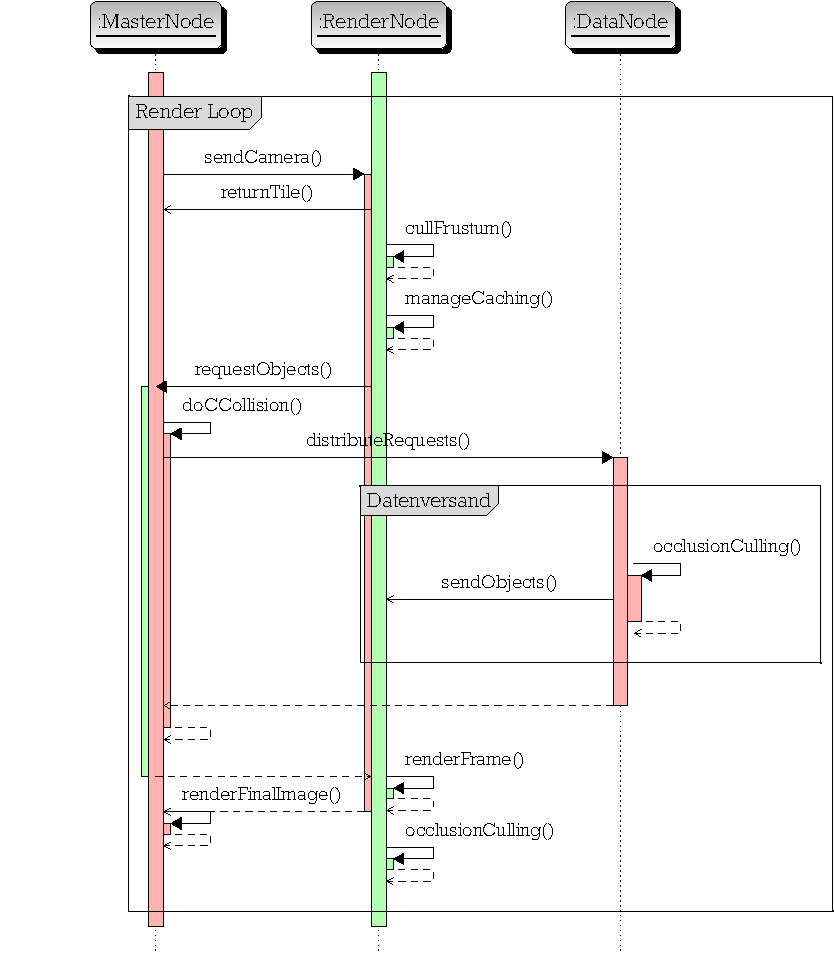
\includegraphics[scale=0.85]{images/seq_diag_render.pdf}
  \captionof{figure}{\label{fig:impl:seqdiagrender}Sequenzdiagramm: Kommunikation für die Render-Schleife}
\end{Bild}

\begin{Bild}
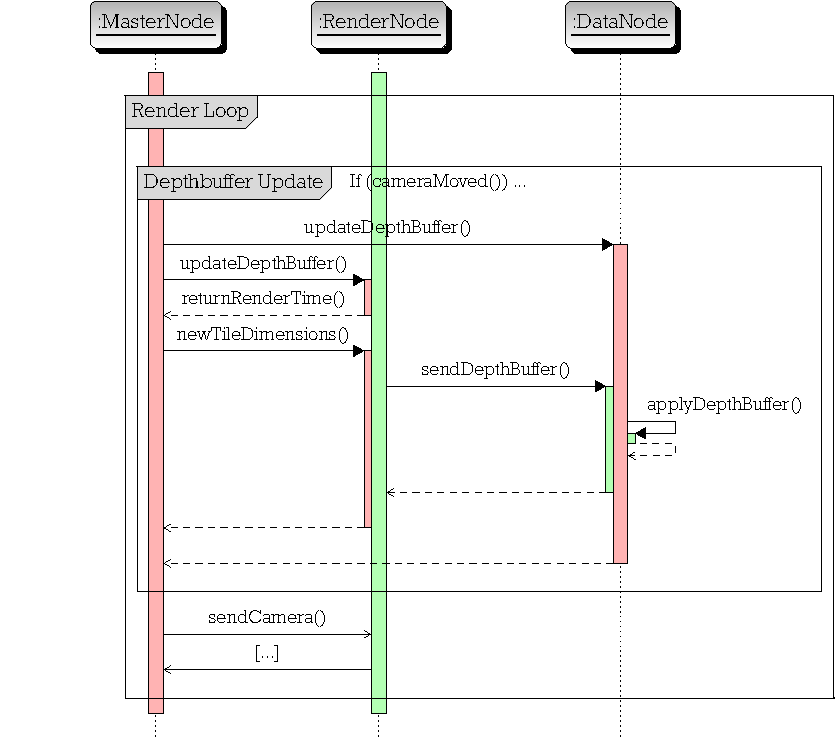
\includegraphics[scale=0.85]{images/seq_diag_depth.pdf}
  \captionof{figure}{\label{fig:impl:seqdiagdepth}Sequenzdiagramm: Kommunikation für ein Tiefenbuffer-Update}
\end{Bild}

%
% EOF
%
